\section{Introduction} 


Nearly all current technologies for applying force and torque between two spacecraft share a disadvantage: they require either propellant or mechanical contact. By using the force between a magnetic field and the electric currents it induces in a conductive target, a new technology known as an induction coupler exploits eddy-current effects to control the relative position and orientation between a chaser spacecraft and a target without mechanical contact. The induction coupler does not rely on familiar magnetic attraction and repulsion, which would require ferromagnetic materials on the target.  In contrast, and induction coupler is broadly applicable for even uncooperative targets, as long as the target includes conductive materials, as is generally the case for spacecraft.

An induction coupler creates actuation force by producing a time-varying magnetic field that induces eddy-currents  through the conductive materials in a target. The coupler's magnetic field then exerts a force on these currents and thus the target. The coupler requires no mechanical contact with a target, nor does it demand cooperation from the target. The coupler operates on electricity alone, enabling close-proximity navigation without propellant. Because most satellites include conductive material in their structure-notably aluminum honeycomb with aluminum facesheets, aluminum isogrid, and aluminum truss elements-induction couplers may be the closest thing we have to science fiction's tractor beam: a device that can produce contactless force on an uncooperative target. It can also be thought of as a contactless momentum-transfer actuator.

Induction couplers show promise for spaceflight applications, offering three major advantages. First, the force associated with magnetic fields across meter-scale distances can dominate gravity, aerodynamic drag, and other effects, which are far less pronounced in orbit than in a terrestrial environment. Second, fully deployed spacecraft are fragile and rarely offer straightforward means for mechanical grappling; so, the ability to interact without the potential for contact damage is valuable. Third, induction couplers offer the ability to maneuver without propellant, eliminating risks associated with thruster-plume impingement \cite{BaerwaldR.S.1977}
and extending the useable lifetime of the chaser spacecraft.
A small spacecraft could use induction couplers to control its motion relative to a much larger target like the International Space Station (ISS), crawling just above the target's surface without ever touching. This on-orbit inspection technique resembles the operations concept for underwater robots that now inspect pipelines and shipwrecks \cite{Whitcomb2000}.

 Systems of induction couplers can conditionally produce force in any direction relative to the target, for example both tangential and perpendicular to a surface on that target. Therefore, a chaser spacecraft generating a time-varying magnetic field can produce forces in all three translational degrees of freedom. Two induction couplers separated by a moment arm can also produce torques, for complete 6DoF actuation.
%% TODO - move this. Perhaps include figures for this. 
There are two ways for an induction coupler to generate its changing magnetic fields and resultant force: permanent magnets that move mechanically and electromagnets driven by time-varying currents. Each type of magnet is especially good at producing forces in different directions. For example, a single electromagnet with a sinusoidal driving current always repels the target. \cite{Reinhardt2012}.  A rotating permanent magnet is effective in producing a shear force, i.e. a force that lies in the plane of a surface.  Replicating the pure repulsive force of an electromagnet with a permanent magnet would require either a linear actuator or a complicated set of linkages. Therefore, a spacecraft that implements induction couplers likely incorporates a combination of permanent magnets and electromagnets. This paper focuses primarily on a free-flyer inspection vehicle which uses those shear forces to move along its target. 

%Ben: I'm pretty sure this is unecessary
%\begin{figure}
%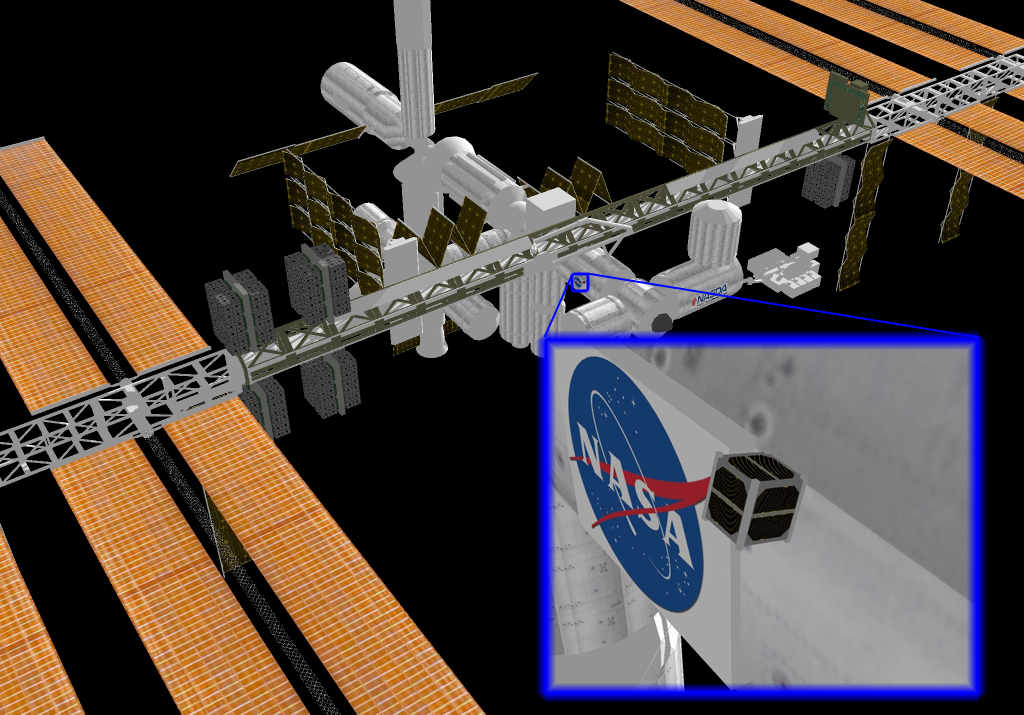
\includegraphics[width = 6cm, height = 6cm %{figures/Induction_Coupler_Overview_Diagram.jpg}
%\label{fig:inspector_diagram}
%\caption{A spacecraft can use an induction coupler with three spinning magnets to create actuation force and torque}
%\end{figure}
 
Current interest in on-orbit servicing (OOS) is a strong motivation for advancing induction coupler technology. \cite{Ambrose2012}
 One of the more compelling use cases is that of a small inspection vehicle whose interactions with the target do not produce significant motion in that target-for example, an ISS inspection vehicle. 
 
An inspector spacecraft with induction couplers can fulfill a number of functions including verifying the state of health, performing mechanical tasks, or providing communications and other logistical support for astronauts during extravehicular activity (EVA). It may be possible for the eddy currents use for locomotion to detect mechanical damage, as is currently done on some aircraft. \cite{Yang2010}
 This paper focuses on the International Space Station (ISS), but a similar inspection spacecraft could enable unique OOS missions to inspect and repair other large satellites.

The inspection spacecraft described here uses induction couplers to pull itself along the aluminum exterior of the ISS, maintaining a separation distance of a few centimeters. In doing so, it acts like a damage-inspection Roomba,\cite{Tribelhorn2007}
 canvassing the surface and automatically detecting damage from micrometeorite strikes. An alternative operations concept is one in which the inspector is controlled directly by an astronaut to evaluate some region of interest and possibly use an attached robotic arm to effect a repair. In yet another concept, the spacecraft acts like an extra pair of hands during an EVA, remaining near an astronaut and holding tools. NASA's Robonaut and the Mobile Servicing System (the Canadian robotic arm on ISS) have demonstrated the value of such a capability but are limited by rails to specific locations. \cite{Ambrose2012}
The ability to traverse the exterior of the ISS without being constrained to travel on rails, attach to specific hard points, or manage a finite propellant supply can free up one of the most valuable resources on the ISS, astronaut time, and may augment astronaut safety.Such a vehicle is primarily concerned with regulating planar motion along the surface of the target and stabilization of out-of-plane translation. This paper describes a study of how the in-plane component of that motion can be achieved with induction couplers.

\begin{figure}
\includegraphics[width = 6cm, height = 6cm ]{figures/iss_inspector.jpg}
\caption{A chaser traverses the surface of the ISS using induction couplers}
\label{fig:iss_inspector}
\end{figure}
 
This paper gives an overview of alternative technologies for contactless space actuation \ref{sec:alt_tech} and the different methods of modeling eddy-current forces \ref{sec:ec_forces}. Section \ref{sec:simple_model} makes simplifying assumptions on the model for planar inspection and experimental data confirms the validity of those models and gives real-life numbers on power consumption and force output in section \ref{sec:experiment}. Section \ref{sec:system} finds a full 6-DoF model of an induction coupler system, describes the important properties of the system, and simulates a simple application.   




